\section{Background and Motivation}
\label{sec:motivation}

In this section, we present measurement results that demonstrates the network performance and resource overhead of different optional network channels. We focus on network throughput and latency when containers are located in the same or different hosts. 
We choose two kinds of hosts: physical machines and VMs in public clouds.

\subsection{Running environments of containers}

\begin{figure}[t!] 
     \centering 
     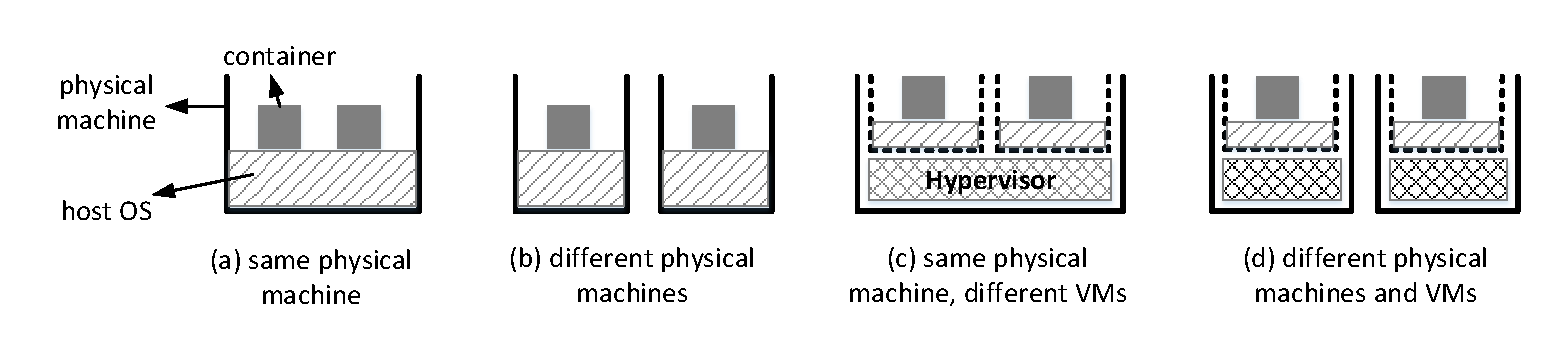
\includegraphics[width=2.8in]{figures/deployment-cases} 
    \caption{\label{fig:deploy-cases} Representitive running environments of containers.} 
\end{figure} 

\subsection{TCP/IP's ineffiency}

\subsection{RDMA's ineffiency}

\subsection{Shared-memory's limitation}


\harry{The point of this section: showing that different network channels have performance advantage in different scenarios.}

\subsection{The measurement setup}
(1) two bare metals: 40Gbps NICs.
(2) two VMs on top of the two bare metals.
(3) two VMs from Azure or EC2.

\subsection{Intra-host Network Performance}

\para{Throughput}

Three points: (1) TCP throughput is limited; (2) the bottleneck is CPU rather than memory bus for TCP/IP; (3) the bottleneck is NIC CPU for RDMA. (4) For intra-host cases, shared memory has the best performance.

Figure 1: throughput of single src-dst pair. Bar figure: x-axis: TCP/IP, RDMA and shared memory; y-axis: throughput;

Figure 2(a): throughput of multiple src-dst pair. Line figure: x-axis: number of pairs,; y-axis: throughput; Four lines: TCP/IP, RDMA, shared memory and memory bus.

Figure 2(b): CPU utilization. Line figure: x-axis: number of pairs,; y-axis: CPU utilization; Three lines: TCP/IP, RDMA, shared memory.

Figure 2(c): NIC CPU utilization. Line figure: x-axis: number of pairs,; y-axis: NIC CPU utilization; Three lines: TCP/IP, RDMA, shared memory.


\para{Latency}
Two points: (1) going through OS stack is increasing network latency; (2) The bottleneck is on system calls.

Figure 3: The stacked bar chart showing the total latency of TCP/IP, RDMA, shared memory and their components.


\subsection{Inter-host network performance}

points: (1) inter-host is generally worse than intra-host, so people have intensive to pack; (2) RDMA has the best performance in inter-host case;

Figure 4: the throughput of single src-dst pair in bare metal. Bar figure: x-axis: TCP/IP, RDMA and shared memory; y-axis: throughput;

Figure 5: the throughput of single src-dst pair in clouds. Bar figure: x-axis: TCP/IP, RDMA and shared memory; y-axis: throughput;
